

\documentclass[11pt,a4paper]{article}
\usepackage{amsmath}
\usepackage{amssymb}
\usepackage{enumitem}
\usepackage{amsthm}
\usepackage{MnSymbol}
\setlength{\parindent}{0pt}
\usepackage[utf8]{inputenc}
\usepackage{listings} [python]
\usepackage{url}
\usepackage{bussproofs}
\usepackage{rotating}
\usepackage{tikz}
\usepackage{hyperref}

\newtheorem{theorem}{Theorem}[section]
\newtheorem{corollary}{Corollary}[theorem]
\newtheorem{lemma}[theorem]{Lemma}
\newtheorem{mydef}{Definition}

%opening


\newcommand{\lto}{\supset}
\newcommand{\some}{\Diamond}
\newcommand{\all}{\Box}

\newcommand{\tall}[1]{\left[ #1 \right]}
\newcommand{\tsome}[1]{\left\langle  #1 \right\rangle}

\newcommand{\eall}{\mathbf{K}}
\newcommand{\esome}{\mathbf{P}}

\newcommand{\sand}{\; and \;}
\newcommand{\sor}{ \; or \;}
\newcommand{\sneg}{not \;}
\newcommand{\sto}{\Rightarrow}
\newcommand{\negmodels}{\nvDash}


\begin{document}

%\maketitle



\section*{Exercise 31}
\begin{quote}
Axioms expressing relations between modalities:
\begin{equation*}
\mathcal{F} \models \all_2 A \lto \all_1 A
\end{equation*}
whenever in $\mathcal{F}:=\langle W, R_1, R_2 \rangle$ we have:
$R_1$ is a sub-relation of $R_2$ (i.e. $R_1 \subseteq R_2$). \\
The inverse task is even more important:
To find axioms that characterize given semantic connections between relations.
$R_1$ is a sub-relation of $R_2$, in a multi-relation frame $\mathcal{F}$, whenever
\begin{equation*}
\mathcal{F} \models \all_2 A \lto \all_1 A
\end{equation*}
\end{quote}


Let $\mathcal{F}:=\langle W, R_1, R_2, \dots R_n \rangle$ be a frame for $n \in \mathcal{N}$.
\begin{itemize}


\item $R_i \subseteq R_j$ implies $\mathcal{F} \models \all_j \varphi \lto \all_i \varphi$ \\
Assume $R_i \subseteq R_j$, for the frame $\mathcal{F}$. Moreover, take an arbitrary model $\mathcal{M}$ based on the frame $\mathcal{F}$. If it is the case that $\mathcal{M},s \nmodels \all_j \varphi$, then clearly $\mathcal{M},s \nmodels \all_j \varphi \lto \all_i \varphi$. Otherwise, $\mathcal{M},s \models \all_j \varphi$, elevated to the meta-level is $\forall t (sR_jt \sto \mathcal{M}, t \models \varphi)$. By assumption we know that $R_i \subseteq R_j$. That is, every world accessible from $s$ by a relation in $R_i$ is also reachable from $s$ by a relation in $R_j$. Since all worlds accessible from $s$ through a relation in $R_j$ satisfies $\varphi$, one clearly obtains $\forall t (sR_it \sto \mathcal{M}, t \models \varphi)$, which returning to a language level results in $\mathcal{M}, s \models \all_i \varphi$.


\item $\mathcal{F} \models \all_j \varphi \lto \all_i \varphi$ implies $R_i \subseteq R_j$ \\
Assume $\mathcal{F} \models \all_j p \lto \all_i p$. Moreover, consider that $\exists e \in R_i \setminus R_j$. Clearly, $e$ must have a state of origin $s$ and a state of destination $t$. Select a model $\mathcal{M}$ based on $\mathcal{F}$ such that $V(p):= W \setminus \{t\}$. Now, elevating $\mathcal{M}, s \models  \all_j p \lto \all_i p$ to the meta level, results in $\forall t (sR_jt \sto \mathcal{M}, t \models p) \sto \forall t (sR_it \sto \mathcal{M}, t \models p)$. Since by assumption $e \nin R_j$ the statement $\forall t (sR_jt \sto \mathcal{M}, t \models p)$ holds. However, $\forall t (sR_it \sto \mathcal{M}, t \models p)$ can not, due to the fact that $sR_it \land \mathcal{M}, t \nmodels p$.


\end{itemize}




\section*{Exercise 32}
\begin{quote}
Characterizing the relation between future and past time:
\begin{enumerate}
\item $\mathcal{F}\models A \lto \tall{P} \tsome{F} A$ iff $\forall s \forall	t (sR_Pt \sto tR_Fs)$
\item $\mathcal{F}\models A \lto \tall{F} \tsome{F} A$ iff $\forall s \forall	t (sR_Ft \sto tR_Ps)$
\end{enumerate}
\end{quote}


Assumptions. For some model $\mathcal{M}$ and some present $s$. The statement 
\begin{itemize}
\item $\mathcal{M}, s \models \tall{P} \varphi$ elevated to the meta-level $\forall t (sR_Pt \sto \mathcal{M}, s \models \varphi)$;
\item $\mathcal{M}, s \models \tsome{P} \varphi$ elevated to the meta-level $\exists t (sR_Pt \sand \mathcal{M}, s \models \varphi)$;
\item $\mathcal{M}, s \models \tall{F} \varphi$ elevated to the meta-level $\forall t (sR_Ft \sto \mathcal{M}, s \models \varphi)$;
\item $\mathcal{M}, s \models \tsome{F} \varphi$ elevated to the meta-level $\exists t (sR_Ft \sand \mathcal{M}, s \models \varphi)$;
\end{itemize}
Hence, given the assumptions above it follows.
\begin{enumerate}
\item $\mathcal{F}\models \varphi \lto \tall{P} \tsome{F} \varphi$ iff $\forall s \forall	t (sR_Pt \sto tR_Fs)$.
\begin{itemize}
\item "$\Longrightarrow$".
This can be shown, by  assuming that $\mathcal{F}\models \varphi \lto \tall{P} \tsome{F} \varphi$ and that $\exists s \exists t (sR_Pt \sand \neg tR_Fs)$. Since by assumption the formula has to hold in every model based on the frame $\mathcal{F}$. Consider the model $\mathcal{M}$, where $V(p):= \{s\}$. Now consider the formula elevated to the meta-level at state $s$, $\mathcal{M},s \models p \sto \forall u (sR_Pu \sto \exists v (uR_Fv \land \mathcal{M},v \models p))$. By assumption, $\neg tR_Fs$ and for all other states $u$, by definition, $\mathcal{M}, u \nmodels p$. Therefore, $ \exists v (uR_Fv \land \mathcal{M},v \models p)$ can not hold. However, by assumption $\mathcal{M},s \models p$ and $\exists t sR_Ft$. That is, the premise of the internal implication holds, but the consequence does not, thus the consequence of the external implication does not hold and thus the whole statement does not hold. Hence, moving back to the language level, one can conclude that $\mathcal{F}\nmodels \varphi \lto \tall{P} \tsome{F} \varphi$. Thereby contradicting the assumption.

\item "$\Longleftarrow$".
Let $\mathcal{F}$ be a frame that satisfies the property $\forall s \forall	t (sR_Pt \sto tR_Fs)$.
If $\mathcal{F} \nmodels \varphi$, then $\mathcal{F}\models \varphi \lto \tall{P} \tsome{F} \varphi$ holds trivially. Otherwise, $\mathcal{F} \models \varphi$. Take an arbitrary model $\mathcal{M}$ based on the frame $\mathcal{F}$ and an arbitrary state $s$. By assumption $\mathcal{M}, s \models \varphi$. Now consider an arbitrary state $t$ accessible from $s$ through $R_P$. Due to the fact that $sR_Pt$, given the assumptions $tR_Fs$. That is, $sR_Pt$ implies $tR_Fs$ and $\mathcal{M},s \models \varphi$. Therefore, from the assumption that $\mathcal{M} \models \varphi$, given an arbitrary state $s$, if a state $t$ is accessible from $s$, there exists a state $u$, namely $s$, at which $\mathcal{M},s \models \varphi$. Or more concise, $\forall t (sR_Pt \sto \exists u (tR_Fu \sand \mathcal{M},u \models \varphi))$, which is exactly the formula $\mathcal{F}\models \varphi \lto \tall{P} \tsome{F} \varphi$ elevated the the mata-level in the respective model and state.

\end{itemize}

\item $\mathcal{F}\models \varphi \lto \tall{F} \tsome{P} \varphi$ iff $\forall s \forall	t (sR_Ft \sto tR_Ps)$.

This is the exact analogue to the previous statement, the only difference is the $P$ and $F$ are switched.

\end{enumerate}


\section*{Exercise 33}
\begin{quote}
Prove that (1) is equivalent to axiom (K) (with $\all$ replaced by $\eall_i$).
\begin{equation*}
(\eall_i A \land \eall_i (A \lto B)) \lto \eall_i B \iff \eall_i(A \lto B) \lto \eall_i A \lto \eall_i B
\end{equation*}
\end{quote}

A nice way to show this fact is to establish that $((A \land B) \lto C) \lto (A \lto (B \lto C))$ and $(A \lto (B \lto C)) \lto ((A \land B) \lto C) $ are CL tautologies. This is sufficient, as 
\begin{equation*}
(\eall_i A \land \eall_i (A \lto B)) \lto \eall_i B \iff \eall_i(A \lto B) \lto \eall_i A \lto \eall_i B
\end{equation*}
can be translated into
\begin{equation*}
\begin{split}
&(((p_{\eall_i A} \land p_{\eall_i (A \lto B)}) \lto p_{\eall_i B}) \lto (p_{\eall_i(A \lto B)} \lto p_{\eall_i A} \lto p_{\eall_i B})) \; \land \\
&((p_{\eall_i(A \lto B)} \lto p_{\eall_i A} \lto p_{\eall_i B}) \lto ((p_{\eall_i A} \land p_{\eall_i (A \lto B)}) \lto p_{\eall_i B}))
\end{split}
\end{equation*}

To take a different approach from the one below, those tautologies are shown by utilising equivalence transformations. That is, 
\begin{align*}
& A \lto (B \lto C) &&  \mathit{Definition \; of \;} \lto&  \\
& \neg A \lor ( \neg B \lor C) && \mathit{Commutativity \; of \;} \lor& \\
& (\neg A \lor \neg B ) \lor C && \mathit{DeMorgan}& \\
& \neg( A \land B ) \lor C && \mathit{Definition \; of \;} \lto& \\
& ( A \land B ) \lto C && & \\
\end{align*}
At every step we have an equivalence transformation. Thus, both $((A \land B) \lto C) \lto (A \lto (B \lto C))$ and $(A \lto (B \lto C)) \lto ((A \land B) \lto C) $ are shown.\\

Alternatively and more cumbersome.
\begin{itemize}
\item "$\Longrightarrow$"
Consider an arbitrary frame $\mathcal{F}$. Where $\mathcal{F} \models (\eall_i \varphi \land \eall_i (\varphi \lto \psi)) \lto \eall_i \psi$. Now take an arbitrary models based on the frame $\mathcal{F}$ and state $s$.
Clearly, $\mathcal{M},s \models (\eall_i \varphi \land \eall_i (\varphi \lto \psi)) \lto \eall_i \psi$. Consider the following cases
\begin{itemize}
\item \textbf{Case 1:} $\mathcal{M}, s\nmodels (\eall_i \varphi \land \eall_i (\varphi \lto \psi))$
\begin{itemize}
\item \textbf{Case 1.1:} $\mathcal{M}, s\nmodels \eall_i \varphi $\\
If this is the case by semantics of "$\lto$", $\mathcal{M}, s\models \eall_i \varphi \lto \eall_i \psi$ holds. Now again by the semantics of "$\lto$" it follows that $\mathcal{M}, s\models \eall_i(\varphi \lto \psi) \lto  \eall_i \varphi \lto \eall_i \psi$ regardless of the evaluation of $\eall_i(\varphi \lto \psi)$.
\item \textbf{Case 1.2:} $\mathcal{M}, s\nmodels \eall_i (\varphi \lto \psi) $\\
By the semantics of "$\lto$", it clearly follows that $\mathcal{M}, s\models \eall_i(\varphi \lto \psi) \lto  \eall_i \varphi \lto \eall_i \psi$ regardless of the evaluation of $\eall_i \varphi \lto \eall_i \psi$.
\end{itemize}
\item  \textbf{Case 2:} $\mathcal{M}, s\models (\eall_i \varphi \land \eall_i (\varphi \lto \psi))$\\
$\mathcal{M}, s \models \eall_i (\varphi \lto \psi)$ means that $\forall t (sR_i t \sto \mathcal{M},s \models \varphi \lto \psi )$ and $\mathcal{M}, s \models \eall_i \varphi$ means that $\forall t (sR_i t \sto \mathcal{M},s \models \varphi )$. Hence, for all states $t$ reachable from $s$ through $R_i$ we have $\mathcal{M}, t \models \varphi$ and $\mathcal{M}, t \models \varphi \lto \psi$. Thus, it follows that $\mathcal{M}, t \models \psi$, leading to $\mathcal{M}, s\models \eall_i \psi$. Therefore, $\mathcal{M}, s\models \eall_i(\varphi \lto \psi) \lto  \eall_i \varphi \lto \eall_i \psi$.
\end{itemize}
\item "$\Longleftarrow$"
Consider an arbitrary frame $\mathcal{F}$. Where $\mathcal{F} \models \eall_i(\varphi \lto \psi) \lto  \eall_i \varphi \lto \eall_i \psi$. Now take an arbitrary models based on the frame $\mathcal{F}$ and state $s$.
Clearly, $\mathcal{M},s \models \eall_i(\varphi \lto \psi) \lto  \eall_i \varphi \lto \eall_i \psi$. Consider the following cases
\begin{itemize}
\item  \textbf{Case 1:} $\mathcal{M}, s \nmodels \eall_i(\varphi \lto \psi)$ \\
By semantics of "$\land$", $\mathcal{M},s \nmodels  (\eall_i \varphi \land \eall_i (\varphi \lto \psi))$ and thus by semantics of "$\lto$" it follows that $\mathcal{M},s \models  (\eall_i \varphi \land \eall_i (\varphi \lto \psi)) \lto \eall_i \psi$.
\item  \textbf{Case 2:} $\mathcal{M}, s \models \eall_i(\varphi \lto \psi)$ \\
\begin{itemize}
\item  \textbf{Case 2.1:} $\mathcal{M}, s \nmodels \eall_i \varphi$ \\
By semantics of "$\land$", $\mathcal{M},s \nmodels  (\eall_i \varphi \land \eall_i (\varphi \lto \psi))$ and thus by semantics of "$\lto$" it follows that $\mathcal{M},s \models  (\eall_i \varphi \land \eall_i (\varphi \lto \psi)) \lto \eall_i \psi$.

\item  \textbf{Case 2.2:} $\mathcal{M}, s \models \eall_i \varphi$ \\
By semantics of "$\land$", $\mathcal{M},s \models  (\eall_i \varphi \land \eall_i (\varphi \lto \psi))$
$\mathcal{M}, s \models \eall_i (\varphi \lto \psi)$ means that $\forall t (sR_i t \sto \mathcal{M},s \models \varphi \lto \psi )$ and $\mathcal{M}, s \models \eall_i \varphi$ means that $\forall t (sR_i t \sto \mathcal{M},s \models \varphi )$. Hence, for all states $t$ reachable from $s$ through $R_i$ we have $\mathcal{M}, t \models \varphi$ and $\mathcal{M}, t \models \varphi \lto \psi$. Thus, it follows that $\mathcal{M}, t \models \psi$, leading to $\mathcal{M}, s\models \eall_i \psi$. Therefore, $\mathcal{M}, s\models  (\eall_i \varphi \land \eall_i (\varphi \lto \psi)) \lto \eall_i \psi$.
\end{itemize}
\end{itemize}
\end{itemize}

\section*{Exercise 34}
\begin{quote}
Prove: $\mathcal{F} \models A5$ iff $\mathcal{F} \models \mathit{negative \;  introspection}$.
\end{quote}

By definition  $\mathcal{F} \models A5$ is  $\mathcal{F} \models \some \varphi \lto \all \some \varphi$. Sine epistemic logic operates over multiple modalities, consider $\mathcal{F} \models \some_i \varphi \lto \all_i \some_i \varphi$ for some arbitrary $i$. Having only defined a correspondence between the epistemic modal operator and the box operator, the first step is to employ the definition of $\some$, i.e. $\some := \neg \all \neg$. Resulting in  $\mathcal{F} \models \neg \all_i \neg \varphi \lto \all_i \neg \all_i \neg \varphi$. Now we can replace (previous exercise) the $\all_i$ with $\eall_i$ to obtain $\mathcal{F} \models \neg \eall_i \neg \varphi \lto \eall_i \neg \eall_i \neg \varphi$, as the version of (A5) in the language of epistemic logic with multiple agents. Therefore, the it remains to show that,
\begin{equation*}
\forall \varphi \in \mathcal{L}_K \; (\mathcal{F} \models \neg \eall_i \neg \varphi \lto \eall_i \neg \eall_i \neg \varphi) \iff \forall \varphi  \in \mathcal{L}_K \; (\mathcal{F} \models \neg \eall_i \varphi \lto \eall_i \neg \eall_i \varphi)
\end{equation*}
where $\mathcal{L}_K$ is the language of epistemic logic with multiple agents.
That is, (A5) is a schemata and therefore $\varphi$ can be replaced by an arbitrary formula. Consider an arbitrary formula $\psi$ and let $\varphi:=\neg \psi$. By (A5) it follows that $ \mathcal{F} \models \neg \eall_i \neg \neg \psi \lto \eall_i \neg \eall_i \neg \neg \psi$, which by propositional reasoning is equivalent to $ \mathcal{F} \models \neg \eall_i \psi \lto \eall_i \neg \eall_i \psi$. Since, $\psi$ is arbitrary, it follows $\forall \varphi  \in \mathcal{L}_K \; \mathcal{F} \models \neg \eall_i \varphi \lto \eall_i \neg \eall_i \varphi$. Similarly, if $\forall \varphi  \in \mathcal{L}_K \; \mathcal{F} \models \neg \eall_i \varphi \lto \eall_i \neg \eall_i \varphi$ then especially $\forall \neg \psi  \in \mathcal{L}_K \; \mathcal{F} \models \neg \eall_i \neg \psi \lto \eall_i \neg \eall_i \neg \psi$, and since $\psi$ arbitrary $\forall \varphi  \in \mathcal{L}_K \; \mathcal{F} \models \neg \eall_i \neg \varphi \lto \eall_i \neg \eall_i \neg \varphi$.


\section*{Exercise 35}
\begin{quote}
Augment this interpretation to represent an additional agent 3 who knows nothing about the weather in Hanoi and Manaus.
\end{quote}

Note: Undirected edges (without arrows) represent two directed edges.
\begin{center}
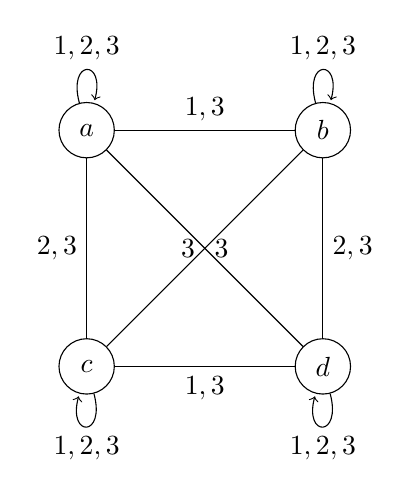
\begin{tikzpicture}
  \tikzset{vertex/.style = {shape=circle,draw,minimum size=2em,inner sep=1pt}}
  \tikzset{edge/.style = {->,- = latex'}}
	\node[vertex] (a) at (0,3) {$a$};
	\node[vertex] (b) at (3,3) {$b$};
	\node[vertex] (c) at (0,0) {$c$};
	\node[vertex] (d) at (3,0) {$d$};
	
	\draw (a) edge[loop above] node{$1,2,3$} (a);
	\draw (b) edge[loop above] node{$1,2,3$} (b);
	
	\path[-](a) edge node [above]{$1,3$} (b);
	\path[-](c) edge node [below]{$1,3$} (d);
   
   	
   	\path[-](a) edge node [left]{$2,3$} (c);
	\path[-](b) edge node [right]{$2,3$} (d);
	
	\draw (c) edge[loop below] node{$1,2,3$} (c);
	\draw (d) edge[loop below] node{$1,2,3$} (d);
	
	\path[-](a) edge node [left]{$3$} (d);
	\path[-](b) edge node [right]{$3$} (c);
   
\end{tikzpicture}
\end{center}
with $V$ being defined as,
\begin{itemize}
\item $V(m):=\{a,c\}$
\item $V(h):=\{a,b\}$
\end{itemize}
Lastly, the new edges have to be added, as not to violate transitivity required by the \emph{positive introspection}.

\section*{Exercise 36}
\begin{quote}
Construct an (infinite) satisfiable set of formulas over p, $\eall_1$, $\eall_2$ and the classical connectives that has no finite Kripke model. (Proof!)
\end{quote}

\textit{[I am terribly sorry for the ugly proof (assuming it is one).]}

Firstly, some syntactic sugar. Let $\esome_x \varphi := \neg K_x \neg \varphi$ for some agent $x$.


Secondly, defining the terminology for the construction of the set of formulas. Consider the following. For all $k \in \mathbb{N}$ with $k \geq 2$,
\begin{equation*}
\varphi_{K_a}(k):= 
\begin{cases}
\eall_a \neg p & \quad k = 2 \\
\eall_a \eall_b \neg p & \quad k = 3 \\
\eall_a \eall_b \varphi_{K_a}(k-2) & \quad otw. \\
\end{cases}
\end{equation*}
and
\begin{equation*}
\varphi_{K_b}(k):= 
\begin{cases}
\eall_b \neg p & \quad k = 2 \\
\eall_b \eall_a \neg p & \quad k = 3 \\
\eall_b \eall_a \varphi_{K_b}(k-2) & \quad otw. \\
\end{cases}
\end{equation*}
where $\varphi_{K}(k):= \varphi_{K_a}(k) \land \varphi_{K_b}(k)$. 
Moreover, 
\begin{equation*}
\varphi_{P}(k):= 
\begin{cases}
\esome_a \esome_b p & \quad k = 2 \\
\esome_a \esome_b \esome_a p & \quad k = 3 \\
\esome_a \esome_b \varphi_P(k-2) & \quad otw. \\
\end{cases}
\end{equation*}
%and
%\begin{equation*}
%\varphi_{P_b}(k):= 
%\begin{cases}
%\esome_b \esome_a p & \quad k = 2 \\
%\esome_b \esome_a \esome_b p & \quad k = 3 \\
%\esome_b \esome_a \varphi_P(k-2) & \quad otw. \\
%\end{cases}
%\end{equation*}
%where $\varphi_{P}(k):= \varphi_{P_a}(k) \lor \varphi_{P_b}(k)$. 
Now, let
\begin{equation*}
\varphi(k) :=\varphi_{K}(k) \land \varphi_P(k)
\end{equation*}
and
\begin{equation*}
\varphi_{*}(k):= (\esome_a \esome_b)^k \varphi(k)
\end{equation*}
where $(\esome_a \esome_b)^k:= \underbrace{\esome_a \esome_b \dots \esome_a \esome_b}_{\mathit{k-times}} $.
Lastly, 
\begin{equation*}
\Gamma_{k}:=  \bigcup_{i=2}^k \{\varphi(i)\}
\end{equation*}
as well as,
\begin{equation*}
\Gamma:=  \bigcup_{i=2}^{\infty} \{\varphi(i)\}
\end{equation*}

Before moving on, an intuitive explanation of the construction. Given a state $s$ the formula $\varphi_K(k)$ ensures that any state reachable by an $ab$-path of length $k-1$, i.e. a path with  $k-1$ steps using the accessibility relations $R_a$ and $R_b$ in alternating fashion, can not be in $V(p)$. While $\varphi_P(k)$ requires that there exists at least one state, accessible from $s$ by an $ab$-path of length at most $k$ where $p$ does hold. However, since any world on the path less then $k$ steps away can not be in $V(p)$, it is not at most $k$ but exactly $k$. Hence, any model satisfying $\varphi(k)$ has to have at least $k$ states. A natural choice for such a model would be the $ab$-path, where the last state will be the only one in $V(p)$. Now as $\Gamma$ is an infinite union of formulas requiring models of increasing size, for any model of a fixed size, it will be possible to find a formula in $\Gamma$ requiring a model of lager size. Moreover, to find a model for $\Gamma$ one has to find a state, where all formulas hold. However, if one attaches all $\varphi(k)$ directly to single state, the requirements imposed by $\varphi_K(k)$ lead to unsatisfiability. Therefore, the sequence $(\esome_a \esome_b)^k$ allows for sufficient buffer, such that one can find a model, without engaging in the complications that arise due the possible interplay of formulas in $\Gamma$. e.g. $\varphi_K(k_1)$ for a large $k_1$ making $\varphi_P(k_2)$ for a small $k_2$ impossible. \\


The first task at hand is to show that $\Gamma$ has no finite model. This shall be split in multiple parts.
\begin{enumerate}
\item For every path $s \leadsto t$ of length $n$ in an epistemic Kripke model $\mathcal{M}$, with two accessibility relations $R_a$ and $R_b$, there exists an $ab$-path $s \leadsto_{ab} t$ of length $m$ such that $m \leq n$. \\

This statement follows directly from transitivity. That is, consider a path $s \leadsto t$ where for $x,y \in \{a,b\}$ and $x \neq y$ there exists a sequence
\begin{equation*}
s_sR_ys_i, s_iR_xs_{i+1}, \dots, s_{j-1}R_xs_j, s_jR_ys_t
\end{equation*}
by transitivity, it follows that $s_iR_xs_j$. Hence, 
\begin{equation*}
s_sR_ys_i, s_iR_xs_j, s_jR_ys_t
\end{equation*}
By replacing the new sequence of steps with the original path one obtains a path of smaller (or equal) size. Moreover, since any sequence of steps in the same accessibility relation can be replaced by a single step, an exhaustive application of this replacement results in an $ab$-path.

(Note: The same holds for the special cases of path over a single accessibility relation. They simply collapse into a single step, which is a trivial $ab$-path)


\item For any model $\mathcal{M} \models \varphi(k)$ for $k \in \{k \mid k>1\}$, it follows that $|W|\geq k$.

From the previous result follows that any arbitrary path between two states, can be replaced by a shorter $ab$-path, thus justifying the focus on $ab$-paths only.

Consider an arbitrary model $\mathcal{M}$ such that there exists a state $s_1$ where $\mathcal{M},s_1 \models \varphi(k)$, which is the same as $\mathcal{M},s_1 \models \varphi_K(k) \land \varphi_P(k)$. Now. since $\mathcal{M},s_1 \models \varphi_K(k) \sand  \mathcal{M},s_1 \models \varphi_P(k)$, it is required that there exists a state $s_{k+1}$ accessible from $s_1$ by an $ab$-path of length $k$, i.e. a path with $k$ steps using the accessibility relations $R_a$ and $R_b$ in alternating fashion, such that $\mathcal{M}, s_{k+1} \models p$. From graph theory, it is known for a graph without weights that, if a vertex occurs twice in a path between two distinct vertices, it can not be the shortest path. Hence, any $ab$-path using a state twice, can be reached by a shorter $ab$-path, and thus no state in this path can satisfy $p$. Therefore, to satisfy $\varphi_P(k)$ one requires an $ab$-path with $k+1$ unique states. Hence, $|W|>k$.

(Note: The two parts of $\varphi_K$, $\varphi_{K_a}(k)$ and $ \varphi_{K_b}(k)$ are required to ensure that the number of alternations determine the truth value of $p$, regardless of which accessibility relation is used for the first step in the $ab$-path. That is, without $ \varphi_{K_b}(k)$ it would be permitted that $s_1R_as_2$ such that $s_1=s_2$.) 

\item For any model $\mathcal{M} \models \varphi_*(k)$ for $k \in \{k \mid k>1\}$, it follows that $|W|\geq k$.

There is some state reachable by an $ab$-path where $\varphi(k)$ holds. To satisfy $\varphi(k)$ at least $k$ unique states are required. Hence, any model satisfying $\varphi_*(k)$ requires at least as many states. 

\item $\Gamma$ has no finite model.


 $\Gamma$ is an infinite union of formulas requiring models of increasing size, for any model of a fixed size, it will be possible to find a formula in $\Gamma$ requiring a model of lager size. 
\end{enumerate}


The second task at hand requires the construction of a model $\mathcal{M}:= \langle W, R_a, R_b, V\rangle$ such that there exists a state $o:=(0,0)$ that $\forall \psi \in \Gamma$, $\mathcal{M}, o \models \psi$.

To that end consider the following model $W:= \mathbb{N}\times \mathbb{N}$ and 
\begin{itemize}
\item $R_a := R_{R_a} \cup O_{R_a} \cup E_{R_a} \cup B_{R_a}$
\begin{itemize}
\item $R_{R_a} := \{(w,w) \mid \forall w \in W\}$
\item $O_{R_a} :=  \bigcup_{k > 1} \{((0,0),(k,1)), ((k,1),(0,0))\} $
\item $E_{R_a} := \bigcup_{j,k > 1} \{((j,1),(k,1))\}$
\item $B_{R_a} :=   \bigcup_{k > 1} \bigcup_{ 1 < i=2n < 3k} \{((k,i),(k,i+1)),((k,i+1),(k,i))\}$
\end{itemize}
\item $R_b :=  R_{R_b} \cup B_{R_b}$
\begin{itemize}
\item $R_{R_b} := \{(w,w) \mid \forall w \in W\}$
\item $B_{R_b} := \bigcup_{k > 1} \bigcup_{ 0 < i=2n+1 < 3k} \{((k,i),(k,i+1)),((k,i+1),(k,i))\}$
\end{itemize}

\end{itemize}
Lastly, $V(p):= \bigcup_{k > 1} \{ (k,3k)\}$.

Again a brief explanation of the structure. $R_{R_a}$ and $R_{R_b}$ ensure reflexivity. 
$O_{R_a}$ connects all paths to a single origin point, while $E_{R_a}$ ensures that $R_a$ remains an equivalence relation. That is, since all branches start with a step in the relation $R_a$, one has to symmetrically connect all worlds in the initial step (to ensure that $R_a$ is euclidean). Lastly, $B_{R_a}$ symmetrically connects each even state with the next one, while $B_{R_b}$ symmetrically connects each odd state with the next one. Hence, no transitive relations are required.\\

Example for $k<4$. (Reflexive edges are not depicted)
\begin{center}
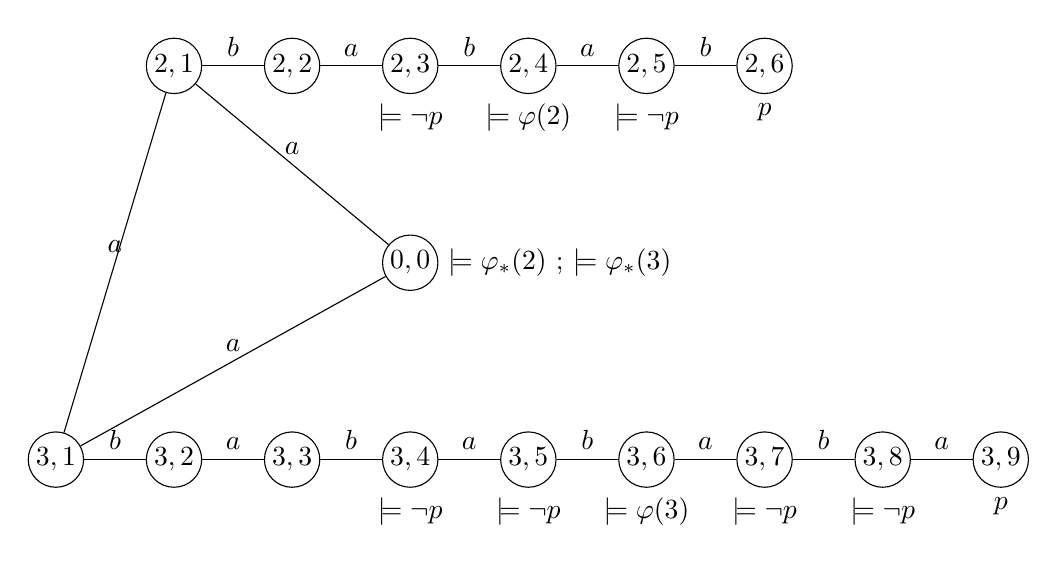
\begin{tikzpicture}
  \tikzset{vertex/.style = {shape=circle,draw,minimum size=2em,inner sep=1pt}}
  \tikzset{edge/.style = {-,- = latex'}}
  
  
  
	\node[vertex] (00)[label=right:$\models \varphi_*(2)$ ; $\models \varphi_*(3)$]  at (5,4) {$0,0$};
	\node[vertex] (21) at (2,6.5) {$2,1$};
	\node[vertex] (22) at (3.5,6.5) {$2,2$};
	\node[vertex] (23) [label=below:$\models \neg p$] at (5,6.5) {$2,3$};
	\node[vertex] (24) [label=below:$\models \varphi(2)$] at (6.5,6.5) {$2,4$};
	\node[vertex] (25) [label=below:$\models \neg p$] at (8,6.5) {$2,5$};
	\node[vertex] (26) [label=below:$p$]  at (9.5,6.5) {$2,6$};
	
	\node[vertex] (31) at (0.5,1.5) {$3,1$};
	\node[vertex] (32) at (2,1.5) {$3,2$};
	\node[vertex] (33) at (3.5,1.5) {$3,3$};
	\node[vertex] (34) [label=below:$\models \neg p$] at (5,1.5) {$3,4$};
	\node[vertex] (35) [label=below:$\models \neg p$] at (6.5,1.5) {$3,5$};
	\node[vertex] (36) [label=below:$\models \varphi(3)$] at (8,1.5) {$3,6$};
	\node[vertex] (37) [label=below:$\models \neg p$] at (9.5,1.5) {$3,7$};
	\node[vertex] (38) [label=below:$\models \neg p$] at (11,1.5) {$3,8$};
	\node[vertex] (39)  [label=below:$p$] at (12.5,1.5) {$3,9$};

    \foreach \from/\to in {00/21,21/31,22/23,24/25, 00/31, 32/33, 34/35, 36/37, 38/39}
    \path[-](\from) edge node [above]{$a$} (\to);

       \foreach \from/\to in {21/22,23/24,25/26, 31/32, 33/34, 35/36, 37/38}
    \path[-](\from) edge node [above]{$b$} (\to);
\end{tikzpicture}
\end{center}

It is to show that for an arbitrary $k>1$, $\mathcal{M},o \models \varphi_*(k)$.
Firstly, $\mathcal{M},o \models (\esome_a \esome_b)^k \varphi(k)$. Consider $(k,2k)$, which is by definition an $ab$-path of length $2k$ away. Hence, one has to test whether $\varphi(k)$ holds at $(k,2k)$, to conclude that $\varphi_*(k)$ holds as $o$. As for $\varphi_{P}(k)$, given the evaluation function $\mathcal{M}, (k,3k) \models p$. which is exactly $k$ alternating steps away from $(k,2k)$. Hence, $\mathcal{M}, (k,2k) \models \varphi_{P}(k)$. Moreover, for $\varphi_{K}(k)$ to hold, all states in all $ab$-paths of length $k-1$ can not satisfy $p$. Given the construction, this means that $\forall s \in \{(k,k+1), \dots (k,3k-1)\}$ it must be that $\mathcal{M},s \nmodels p$, which is clearly the case. Hence, $\mathcal{M},o \models \varphi_*(k)$.
Since, this can be done for an arbitrary $k$, it follows that $\forall \psi \in \Gamma, \mathcal{M}, o \models \psi$.







\end{document}
